\section{Discussion}
\label{sec:disc}

The challenging ocean and meteorological conditions faced as part of
this experiment precluded cycles of week-long operations, as
planned. Nevertheless, we were able to operate for 7 days during the
3-week long deployment. We demonstrated the overall integrative
overall approach to close modeling-sampling-assimilation-tasking cycle
with the goal of improving the skill of oceanographic models by
leveraging observations from AUVs, traditional methods such as
ship-based measurements and opportunistic measurements using low-cost
sensors, and by exploring synergies between dedicated surveys and
opportunistic observations.

Full integration of command and control strategies comprising modeling,
assimilation and adaptive sampling algorithms was demonstrated with the
help of the advanced LSTS software toolchain enabling 24/x operations
with minimal operator’s support. The deployments were performed to
evaluate and test the overall approach in an incremental fashion. The
last days of the deployment demonstrated several iterations of the
closed modeling-sampling-assimilation-tasking cycle. The accuracy of the
predictions of the geostatistical model increased after several cycles,
while the overall prediction errors decreased. However, these results
still lack statistical significance because of the few consecutive
cycles in which the overall approach was tested. We observed that we
never had more than 3 consecutive days of operation.

The dense grid of AUV observations enables post-experiment evaluation
and testing of the assimilation schemes and of the geostatistical model.
While we are still lacking the desired statistical significance of a
long series of consecutive cycles, these post-experiment activities will
lead to a better understanding of the overall procedures and the
identification of improvements, namely the optimization of the
parameters used for the coordinated integration of the algorithms used
in the modeling-sample-assimilation-tasking cycles. We will further
investigate the selection of representative depths for the application
of the sampling algorithm used to find the horizontal projection of the
AUV paths.

This field study provided invaluable lessons in operational procedures,
refinement of adaptive sampling and algorithms, and risk minimization to
operate in an area with dense ship traffic and fishing nets. Our AUVs
were occasionally impacted by strong vertical currents that may have
resulted from the impact of internal waves that are common in the area,
namely in stratified regions (which was the case) and that were observed
with the help of remote sensing imagery during the deployments. Finally,
the results achieved with this deployment provided additional insights
and the motivation to further advance the state of the art in refining
the modeling-sampling-assimilation-tasking cycle with the goal of
improving the skill of oceanographic models. Furthermore, dense grids of
sampled oceanographic data have the potential to fuel developments
targeting existing gaps in modeling skill when different levels of
spatial and temporal resolution are considered \cite{Balaji_2022}.


\begin{figure}[!]
  \centering
  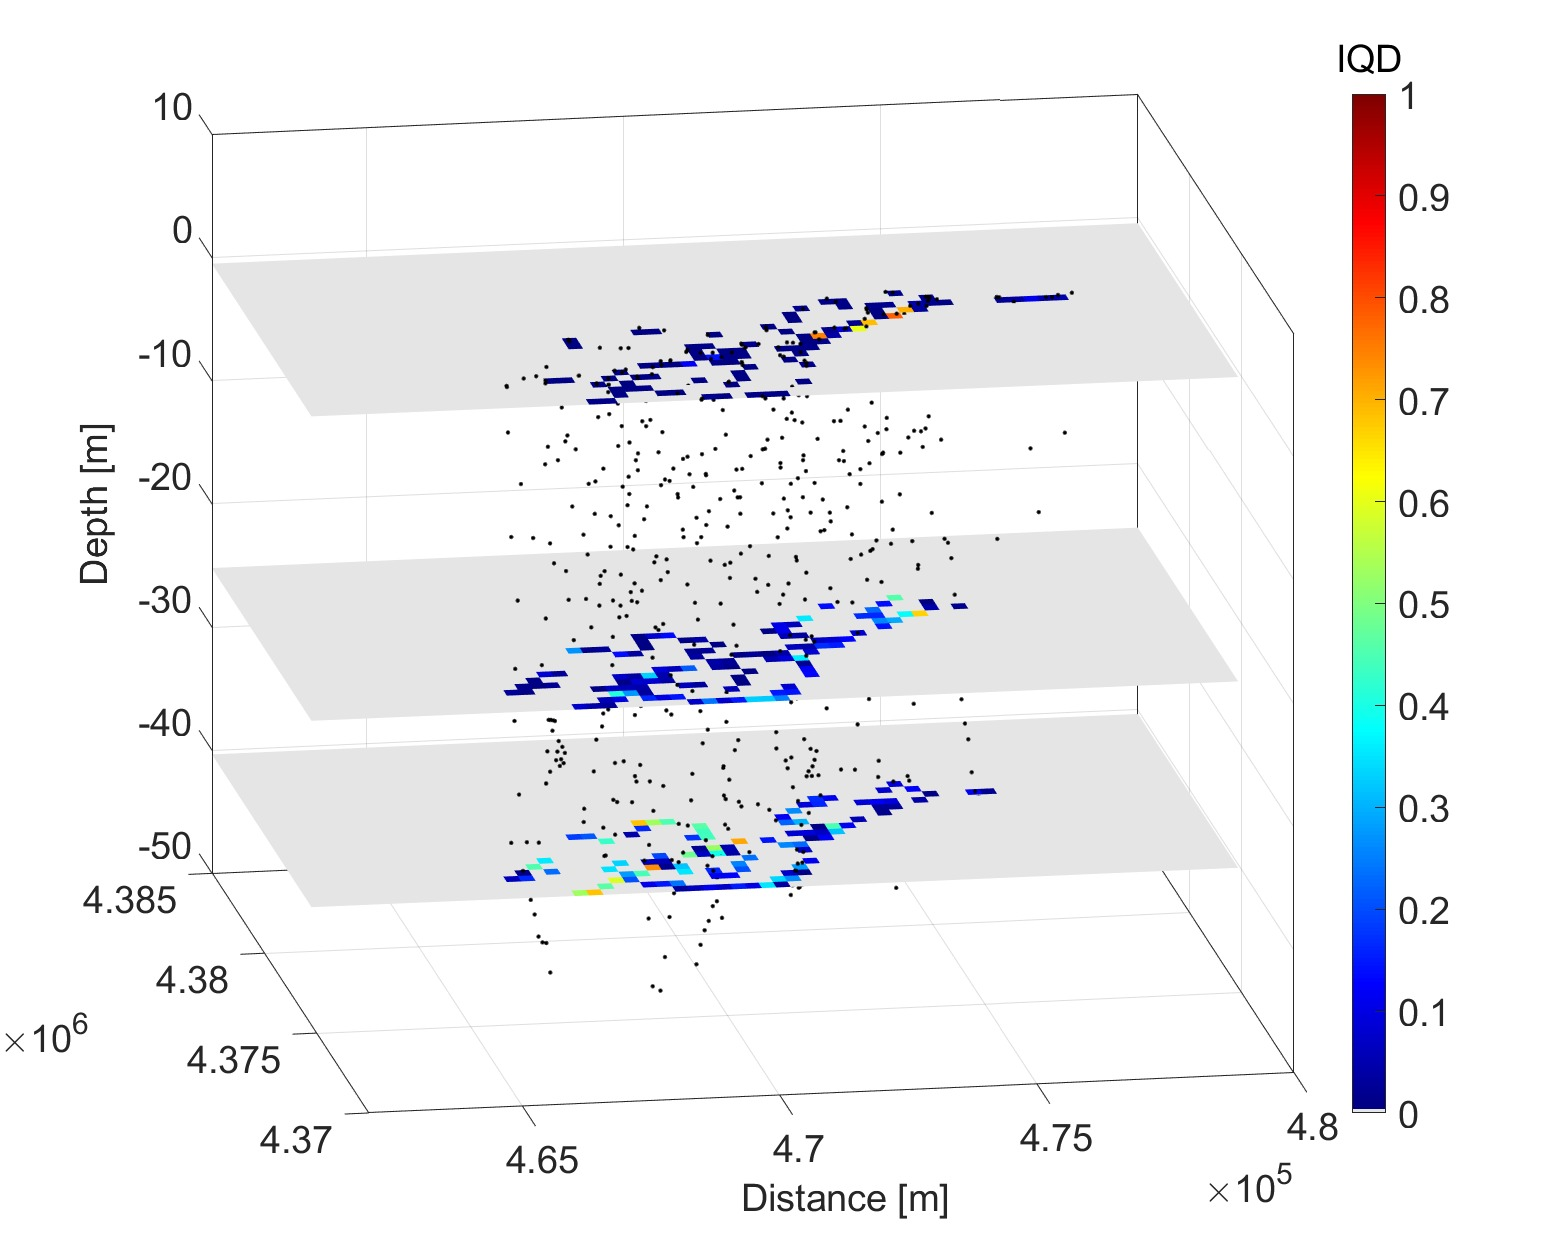
\includegraphics[scale=0.3]{fig/iqd_3D.jpeg}
  \caption{not the final figure}
  \label{fig:iqd_3D}
\end{figure}


